%\section{\texorpdfstring{Backgrounds for $\tauTau$}{Backgrounds for tauTau}}
%\label{sect:bkg}
\subsection{\texorpdfstring{QCD Background Estimation in $\tauTau$ Channel}{QCD Background Estimation in tau-tau Channel}}
In QCD multi-jet events all tau candidates are misidentified jets. Due to the large cross
section and
the poor MC modelling of the tau misidentification rate from jets, the QCD multi-jet contribution in the signal region 
is estimated from data using the ABCD method.
This method relies on different distributions of QCD
in the four exclusive regions labelled as A, B, C (the control regions) and D (the signal region) which are defined in a two-dimensional plane as a function of uncorrelated discriminating variables.
Then the number of QCD events in signal region D can be calculated from the number of QCD events in the control region A multiplied by a transfer factor which is defined as the ratio of the number of QCD events in the control region C to the number of QCD events in control region B $(T=C/B)$.\\
The two discriminating variables used to define regions A, B, C and D are the isolation 
variable and a kinematic variable chosen as \mttwo in search \binone or \SumMT in search \bintwo.  
The definitions of the control regions are summarized in table~\ref{2QCDbg}. \\
\begin{table}
\begin{center}
\begin{tabular}{|c|c|c|c|}
\hline
Region&A& B & C
\\ \hline\hline
\multirow{5}{*}{search \binone} &$\mttwo >90$ & $\mttwo <90$&$\mttwo <90$ \\
&at least 1 loose tau&at least 1 loose tau& loose tau veto\\
&loose-loose loose-medium &loose-loose loose-medium &medium-medium \\
&loose-tight&loose-tight&medium-tight tight-tight\\
&No cut on charge&No cut on charge& OS\\
\hline
\multirow{5}{*}{search \bintwo}&$\SumMT >250$ &$\SumMT <250$&$\SumMT < 250$\\
&at least 1 loose taus&at least 1 loose taus& loose tau veto\\
&loose-loose loose-medium &loose-loose loose-medium &medium-medium \\
&loose-tight&loose-tight&medium-tight tight-tight\\
&No cut on charge&No cut on charge& OS\\
% &misc.MinMetJetDphiPt40$>$1 is relaxed\\
\hline
\end{tabular}
\caption{The control regions used for ABCD method are defined. The $\mindphifour>1$ cut is removed to incraese the statistics.}
\label{2QCDbg}
\end{center}
\end{table}
\\The number of QCD multi-jet events in the control regions is estimated from data after subtraction 
of other SM contributions estimated from MC simulation. The distribution of the transfer factor as a 
function of the search variable is shown in figure~\ref{fig:1QCDbg}. The correlation 
between the two variables used to define the four exclusive regions is marginal, since the ratio plots can be fitted with a straight line using a $pol0$ function. The fit function is also shown in the plots.\\ 
\begin{figure}[!Hhtb]
\centering
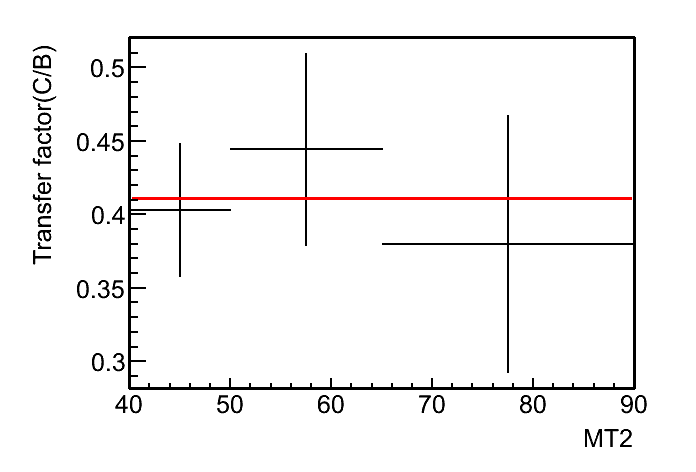
\includegraphics[width=0.49\textwidth]{QCDbginTauTau/Bin1_transferfactor.png}
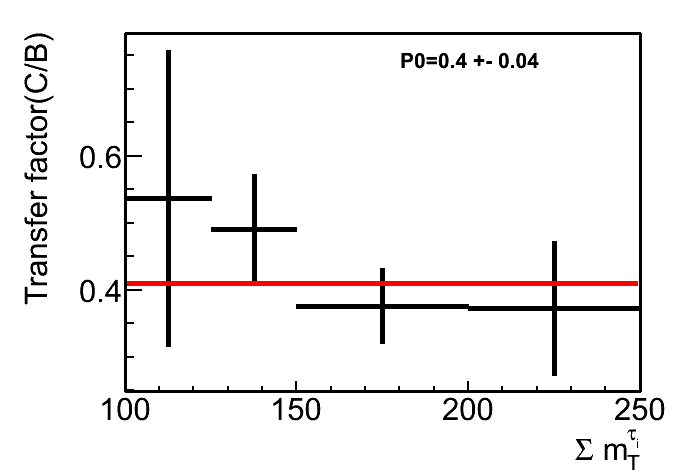
\includegraphics[width=0.49\textwidth]{QCDbginTauTau/Bin2_transferfactor.png} \\
\caption{The distribution of transfer factor as a function of \mttwo (left) and \SumMT (right). A $pol0$ function is used to fit the plots.}
\label{fig:1QCDbg}
\end{figure}


In order to increase the contributions from QCD events, the cut on the $\mindphifour>1$ is removed.
To consider the effect of this cut, a cut efficiency should be taken into account. The 
fraction of QCD events with all selection cuts with respect to the QCD events with all selection 
cuts but the $\mindphifour>1$ are shown in figure~\ref{fig:3QCDbg}.\\
\begin{figure}[!Hhtb]
\centering
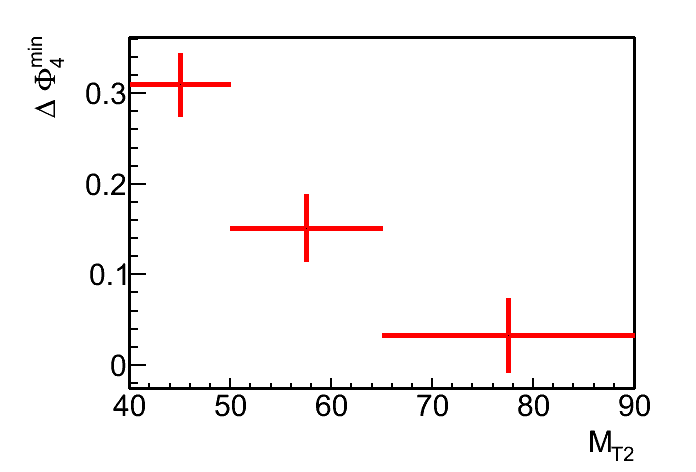
\includegraphics[width=0.49\textwidth]{QCDbginTauTau/Bin1_miscefficiency.png}
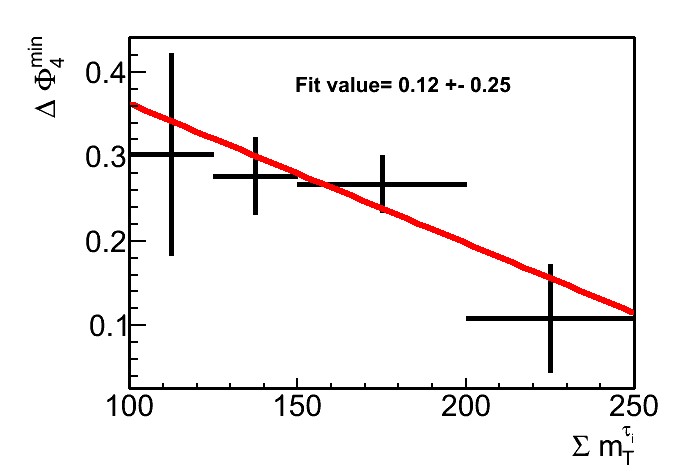
\includegraphics[width=0.49\textwidth]{QCDbginTauTau/Bin2_miscefficiency.png} \\
\caption{ The fraction of QCD events with all selection cuts with respect to the QCD events with all selection 
cuts but the $\mindphifour>1$ as a function of \mttwo (left) and \SumMT (right).}
\label{fig:3QCDbg}
\end{figure}

The value of the cut efficiency 
in the last bin of the left plot is used for the estimation of the 
QCD background events in the search \binone. While for the right plot, the distribution is fitted with a $pol1$ function to 
take into account the fluctuations of the cut efficiencies in the first few bins. Then the cut efficiency extracted from 
this plot is simply defined as the evaluation of the fit function at $\SumMT=250$. [{\bf FIXME} update this with comments from SUSY meeting] It should be noted that, performing such a 
$pol1$ fit function on the left plot would yield to a negative value for the cut efficiency and then it was decided to  
take the value in the last bin as a conservative estimate of the cut efficiency which is used in the final QCD background estimation results. 
\\The results of the ABCD method are summarized in table~\ref{4QCDbg}. A systematical uncertainty on the MC events when subtracting them from data
is also taken into account, to be 25\% of the central value and added in quadrature to the                           
statistical errors. 
\begin{table}
\begin{center}
\scalebox{0.86}{
\begin{tabular}{|l|c|c|c|c|c|c|c|c|}
\hline
 & Sample & RegionA & RegionB & RegionC & T=C/B &$\mindphifour$efficiency& Estimation\\\hline\hline
\multirow{3}{*}{\binone}& Data&10.00 +- 3.16 & 880.00 +- 29.66& 430.00 +- 20.74& \multirow{3}{*}{0.41+-0.04} & \multirow{3}{*}{0.04 +- 0.04}&\multirow{3}{*}{0.09 +- 0.10}\\ \cline{2-5}
&NonQCD(MC)& 4.47+-1.84 & 122.5+-21.46 & 119.86+-20.59& & \\\cline{2-5}
&Data-NonQCD(MC)&5.53+-3.66 & 757.5+-36.61& 310.14+-29.22& & \\\cline{2-5}
\hline\hline
\multirow{3}{*}{\bintwo}&Data & 20.00+-4.47 &723.00+-26.89 &348.00 +- 18.65 & \multirow{3}{*}{ 0.41 +- 0.04} & \multirow{3}{*}{ 0.12+-0.25}&\multirow{3}{*}{0.65 +- 1.4} & \\
\cline{2-5}
&NonQCD(MC)& 6.53+-2.44&78.28+-14.82 & 85.97+-15.89& & \\\cline{2-5}
&Data-NonQCD(MC)& 13.47+-5.1 &644.72+-30.7 & 262.03+-24.51& & \\\cline{2-5}
\hline\hline
\end{tabular}}
\caption{The ingredients needed for the ABCD method are summarized. The quoted 
uncertainties on data are statistical. For the nonQCD(MC) events, the systematical uncertainty  
 is also considered as 25\% of the central value and added in quadrature to the 
statistical errors. This systematical uncertainty is also propagated to the data subtraction.  
The final QCD background estimation results is shown in the last column.}
\label{4QCDbg}
\end{center}
\end{table}
The distributions 
of the search variables are shown in figure~\ref{fig:5QCDbg}. The SM background distributions are taken from MC simulation, except for 
the QCD multi-jet contribution, which is estimated using the ABCD method.
\begin{figure}[iHhtb]
\centering
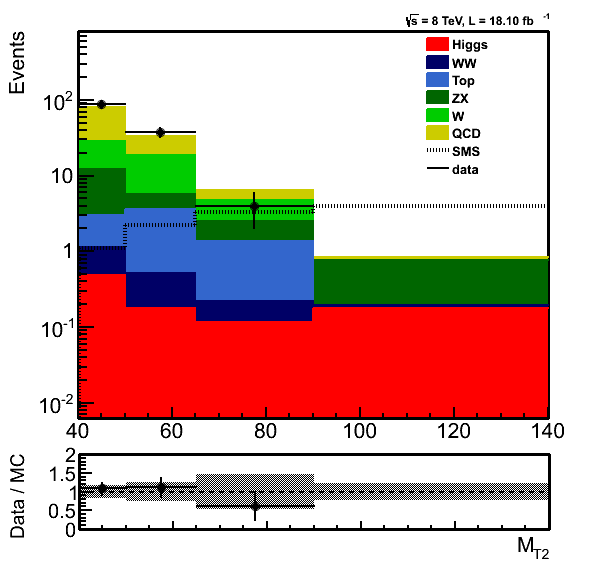
\includegraphics[width=0.49\textwidth]{QCDbginTauTau/Bin1_QCDdatdriven.png}
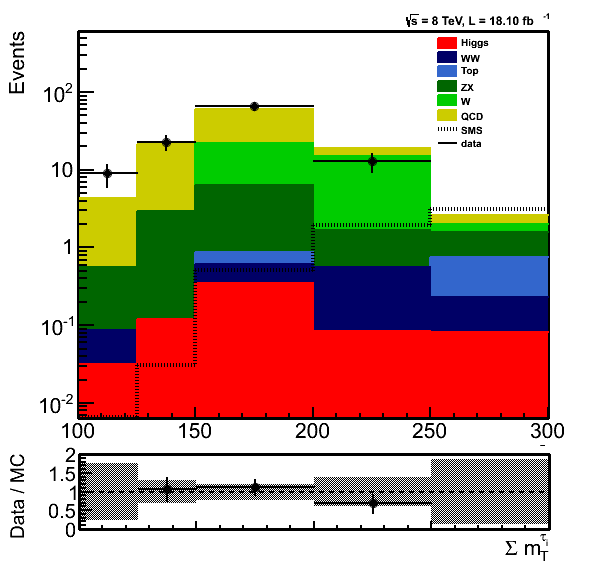
\includegraphics[width=0.49\textwidth]{QCDbginTauTau/Bin2_QCDdatdriven.png} \\
\caption{The distributions of the \mttwo (left) and \SumMT (right) before the requirement on the given variable
is applied. The QCD multi-jet contribution is estimated from data using the ABCD method.}
\label{fig:5QCDbg}
\end{figure}


